\documentclass[conference]{IEEEtran}
\IEEEoverridecommandlockouts
\usepackage{cite}
\usepackage{amsmath,amssymb,amsfonts}
\usepackage{algorithmic}
\usepackage{graphicx}
\usepackage{textcomp}
\usepackage{graphicx}
\graphicspath{ {./images/} }
\usepackage{multicol}
\usepackage{xcolor}
\usepackage{natbib}
\usepackage{graphicx}
\usepackage{listings}
\usepackage{xcolor}
\usepackage[utf8]{inputenc}
\usepackage{hyperref}
\def\BibTeX{{\rm B\kern-.05em{\sc i\kern-.025em b}\kern-.08em
    T\kern-.1667em\lower.7ex\hbox{E}\kern-.125emX}}

\begin{document}

\title{
Locating vertically and horizontally aligned points in XY Cartesian space.\\
}

\author{\IEEEauthorblockN{Ritu Kiran Murmu}
\IEEEauthorblockA{IIB2019025}
\and
\IEEEauthorblockN{Atithi Kumari}
\IEEEauthorblockA{IIB2019026}
\and
\IEEEauthorblockN{Shahid}
\IEEEauthorblockA{IIB2019027}
}

\maketitle

\textbf{\emph{{Abstract}: In this paper, we have designed an algorithm to locate vertically aligned points and horizontally aligned points with XY coordinates in a Cartesian space. The algorithm will result in all the starting and ending points of lines which are formed vertically and horizontally.
}}\\

\section{\textbf{Introduction}}
\noindent We have been given N points in the Cartesian space. In order to find the horizontal and vertical aligned points polynomials, we need to locate all the vertical and horizontal lines in the cartesian space. \\
\\
\noindent We know that to make a line, we need at least 3 points in XY Cartesian space. So, by using this condition, we are going to find all the horizontal and vertical lines in the Cartesian space. The vertical lines can be found by grouping those points which have same x-coordinates, and horizontal lines by same y-coordinates.\\
\\
\textbf{Map} Maps are associative containers that store elements formed by a combination of a key value and a mapped value, following a specific order.\\
\\In a map, the key values are generally used to sort and uniquely identify the elements, while the mapped values store the content associated to this key. The types of key and mapped value may differ, and are grouped together.\\

The time complexity to store values in map is  O(Log n) while for unordered map, it is O(1) on average. \\
\\
\\
\noindent The algorithm  is described in detail in \textbf{part II}.\\
\section{\textbf {Algorithm Description and Analysis}}

\noindent  Solution is based on the hash map as we have to locate the horizontal and vertical align line.\\

\noindent We have used simple logic  for vertical align point general form x = K. The x axis has the equation y = 0 taken as reference. And same for horizontal align pont general form y=k.\\
\\\textbf{Data Structures Used:}

\begin{itemize}
\item	Map of vector to store Points
\item	Map of vector to store the set of Points\\
\end{itemize}

\begin{enumerate}
\item Generated the random integer value greater than 50 for no. of  point.\\

\item Run the for  loop no. of points time and generated the x , y coordinate for the point.\\

\item In the hash map for the vertical align point store the y coordinate value corresponding to the given x key.\\

\item In the hashmap for the horizontal align point store the x coordinate value corresponding to the given y key.
\\

\item Traverse the map for  x key if more than or equal to  3 y coordinates are available print the start and end point of the vertical align point. \\

\item Traverse the map for  y key if more than or equal to  3 x coordinates are available print the start and end point of the horizontal align point.
\\ 

\end{enumerate}
\textbf{For example} Let there be 10 points,\\
            (0 ,  4) , (4 , 8) , (6 , -6) (-2,-8), (3 , 4) , (3 , -6) , (-1 , 4) , (-13 , -6) , (-8 , -6 ), (3 , 5)\\
\\The horizontal lines formed by given points are: - \\
     {(0 , 4),(3 , 4),(-1 , 4)}\\
     {(6 , -6),(3 , -6),(-8 , -6),(-13 , -6)}\\
\\The vertical lines formed by given points are: -\\
     {(3 , 4),(3 , -6),(3 , 5)} \\
\\As the start and points of lines are our output, so the output for the set of points will be: -\\
\\ (0 , 4) (-1 , 4)
\\ (6 , -6) (-13 , -6)\\
\\(3 , 4) (3 , 5)\\

\section{\textbf{Pseudo Code}} 

\lstset { %
    language=C++,
    backgroundcolor=\color{black!5},
    basicstyle=\footnotesize,
}

\begin{lstlisting}

Int:
Function main()
    map<int,vector<int> > mx;
    mx[x].push_back(y);
    
    for( const auto& pair : mx )
        {
            int s=0;
            int min =INT_MAX;
            int max= INT_MIN;
            for( double d : pair.second )
          
          {   
            if(d > max)
               max=d;
            if(d<min)
               min=d;
            s++;
          }
          
          if(s>=3)
            {
              print (pair.first "," min" " 
                    pair.first "," max) 
                    
              print("\n")
            }
            
        }



\end{lstlisting}

\medskip

\section{\textbf {Time Complexity}}
\noindent The time complexity will be equal to O(nlogn).

T(n) = O(n) * log(n) +c\
\begin{figure}[htp]
    \centering
    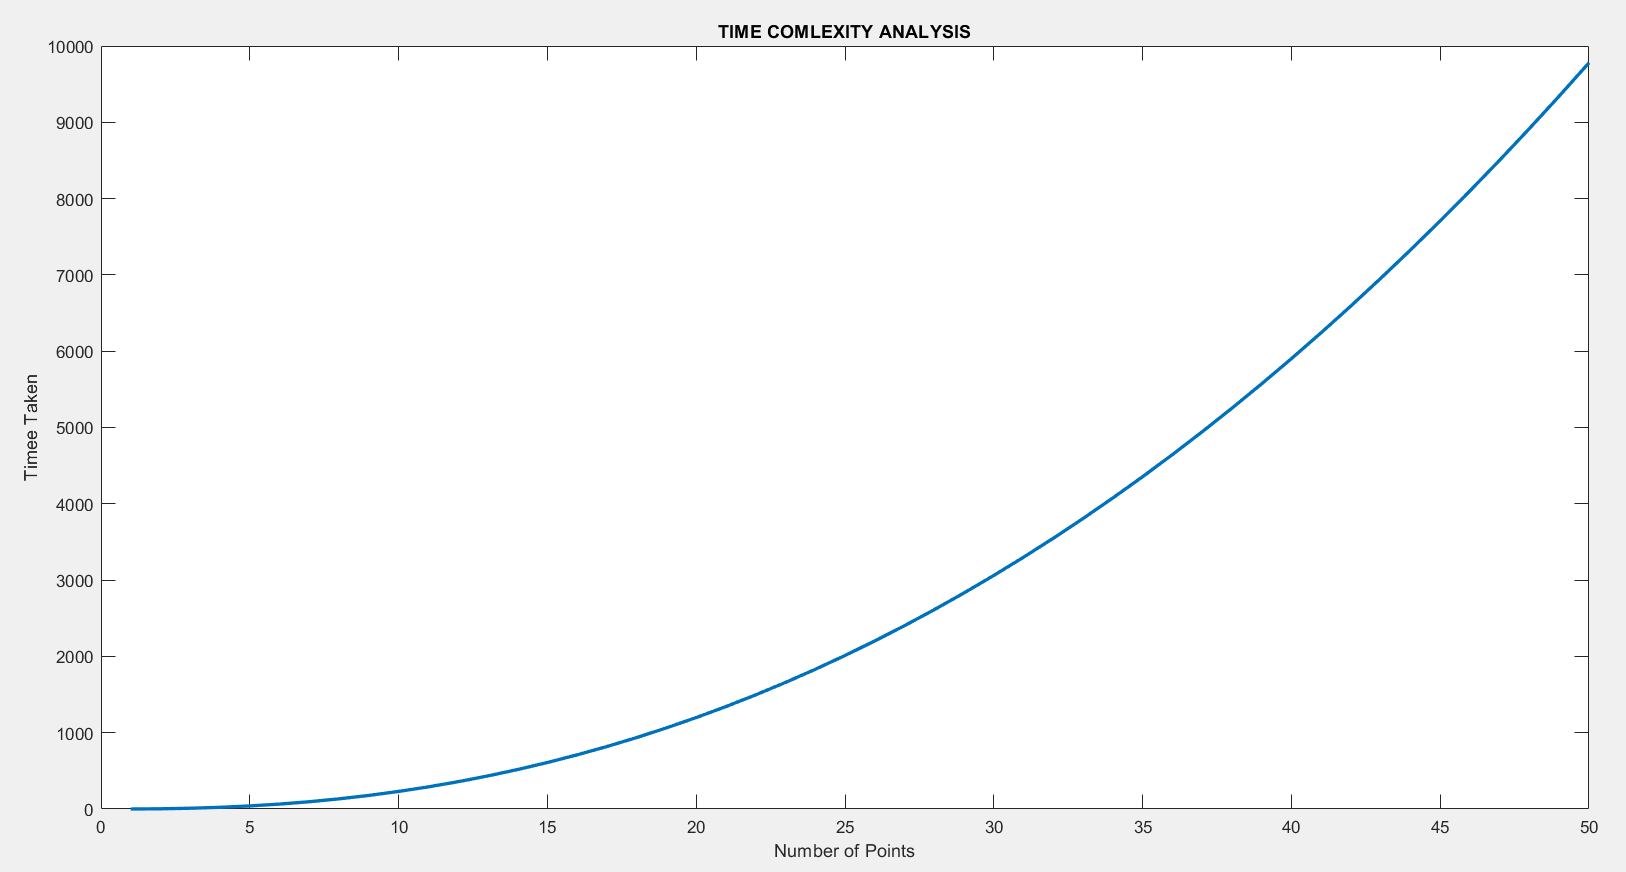
\includegraphics[width=8cm, height=7cm]{daa_3/images/Time Complexity.png}
    \caption{Time complexity curve}
    \label{fig:Time Complexity.png}
\end{figure}

\section{\textbf {Auxiliary Space Complexity}}
\noindent The space complexity of the program is O(n). This is because we are using vectors to store the points.

\begin{figure}[htp]
    \centering
    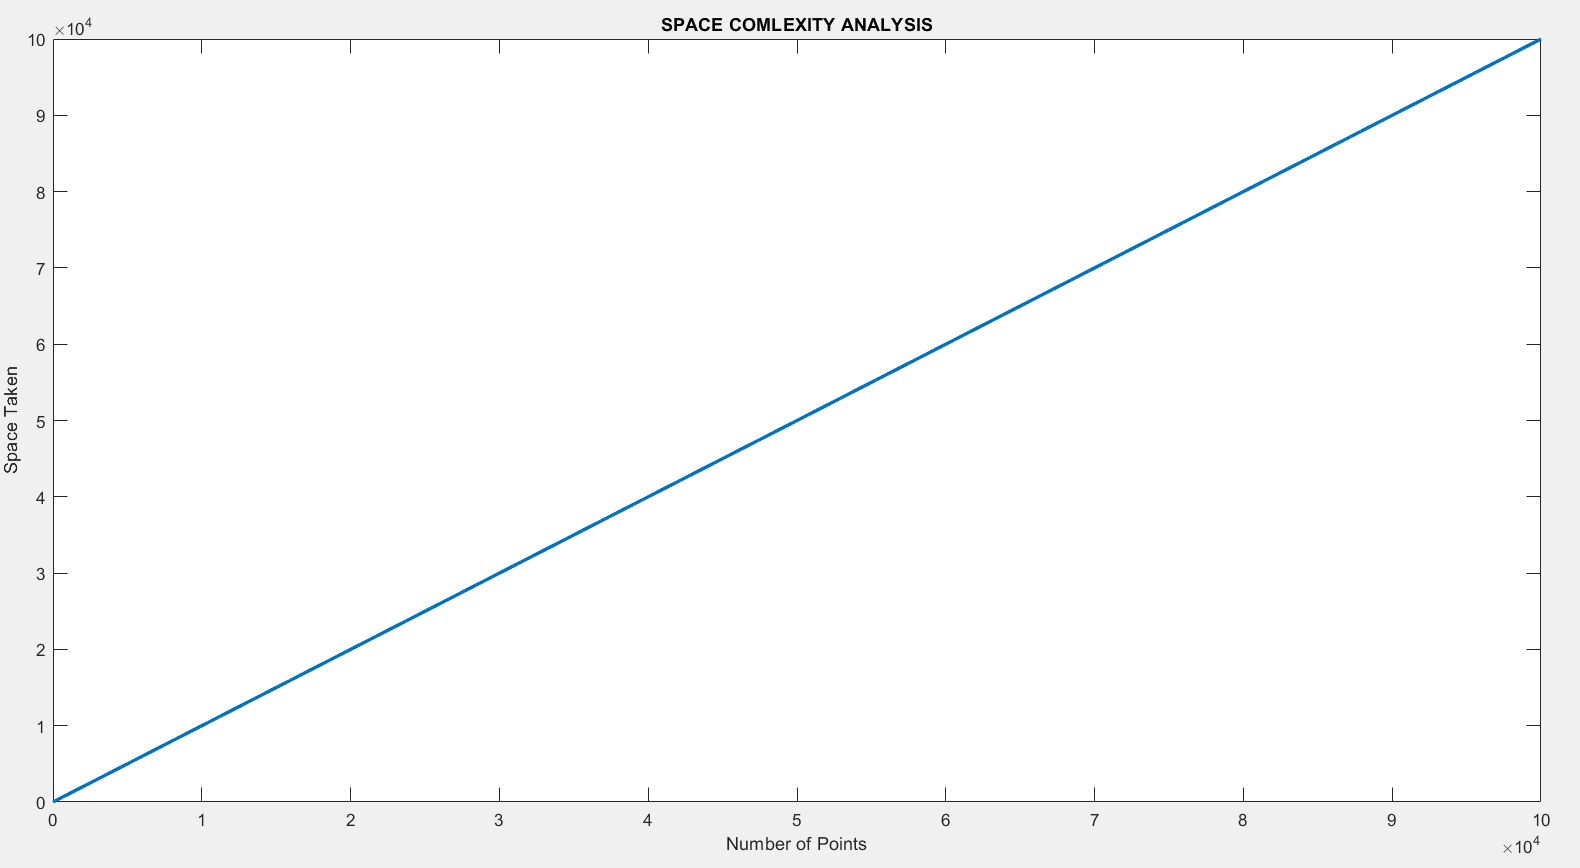
\includegraphics[width=8cm,height=7cm]{daa_3/images/Space Complexity.png}
    \caption{Space complexity curve}
    \label{fig:spacecomplexity.png}
\end{figure}

\section{\textbf {Conclusion}} 
\noindent To find the horizontal and vertical align point we have used the hashmap to store the y or x value to x or y key. Time complexity for this program is nlogn and space complexity is n.\\

\section{\textbf {References}} 

\begin{enumerate}

\item \href{https://www.geeksforgeeks.org/map-of-vectors-in-c-stl-with-examples/}{Map of vector}\\

    
\item  \href{https://www.varsitytutors.com/hotmath/hotmath_help/topics/horizontal-vertical-lines}{Horizontal and vertical lines} \\

\end{enumerate}

\end{document}
